\chapter {Implementación}
    \section {El dominio de las frecuencias}
    \section {Distribución de frecuencias}
    \section {Similitudes en la distribución de frecuencias}
    \section {Generación melódica}
    \section {Evolución creativa}
    


\section{Clasificación de melodías}


\subsection{Descripción del conjunto de entrenamiento}
\paragraph{La base de conocimiento cuenta con un total de 165 melodías, distribuidas de la siguiente forma:}


%\input{implementacion/knowledgebase.lst}

\subsection{Medición de la influencia entre compositores}
\paragraph{Para determinar si el sistema es capaz de identificar el compositor original de una melodía y que ta}

\begin{figure}[h]
    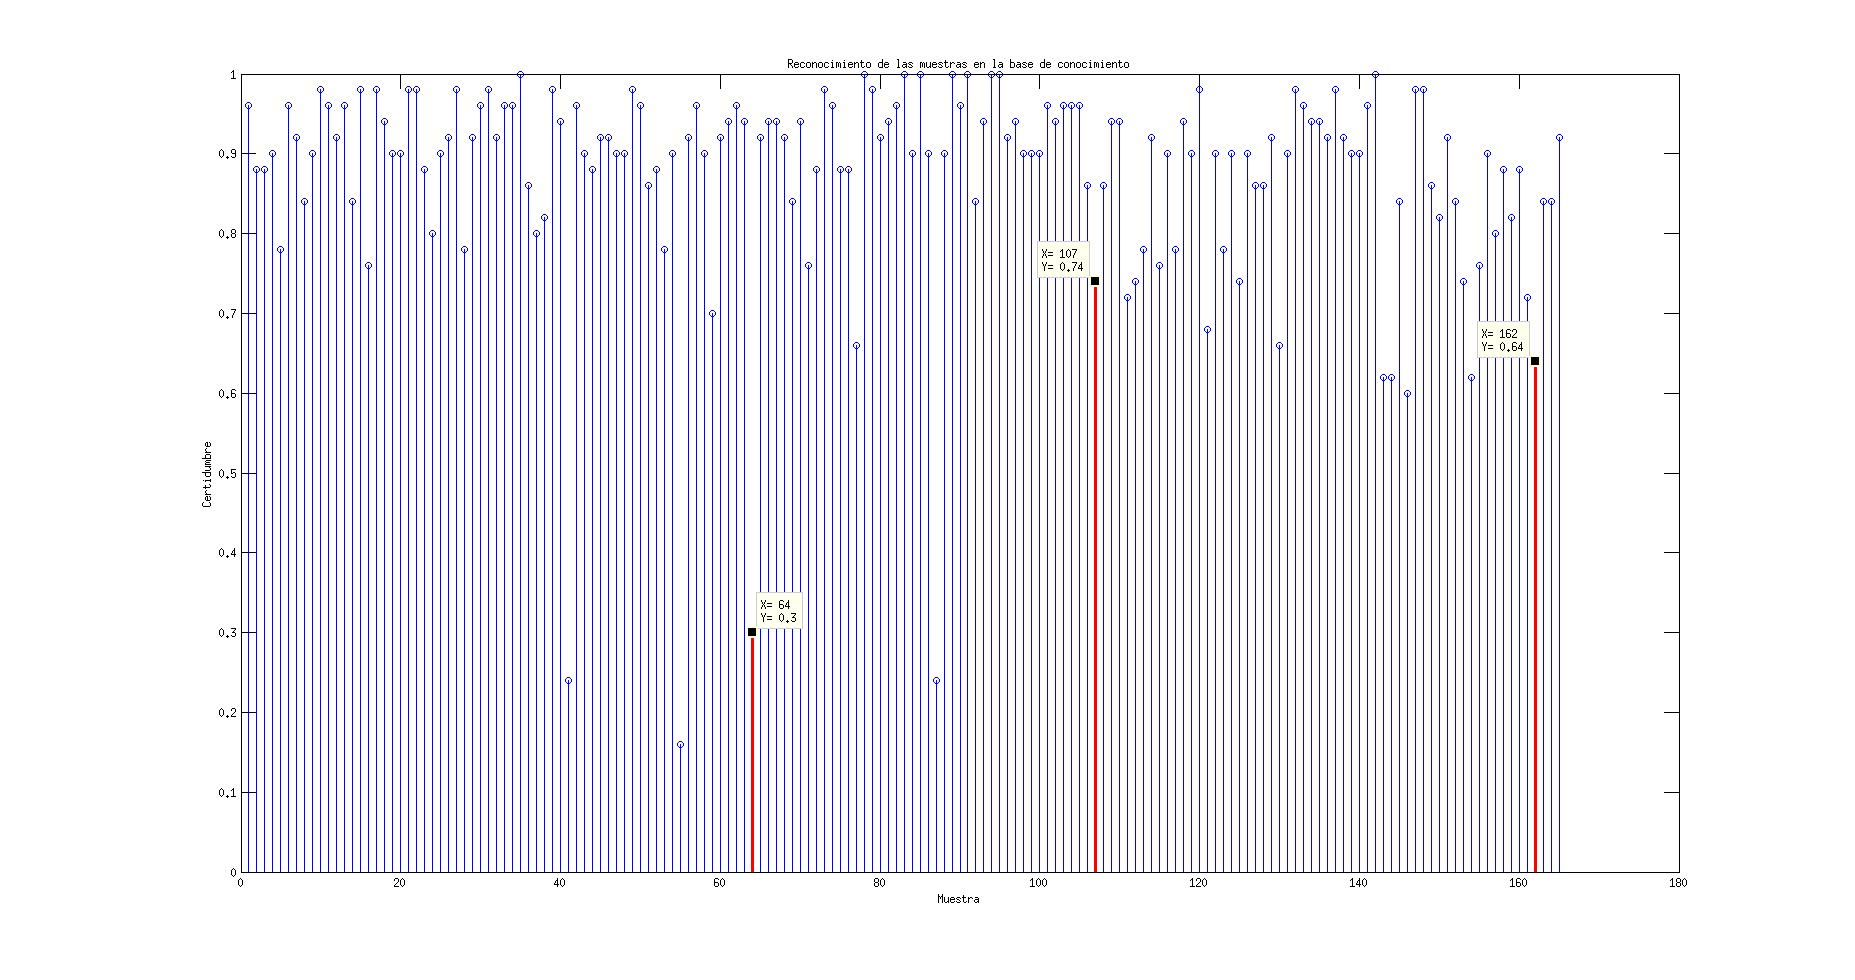
\includegraphics[width=0.9\textwidth]{implementacion/img/covers_kbq.jpg}
    \caption{Certidumbre en el reconocimiento correcto de las melodías del conjunto de entrenamiento}
\end{figure}

\begin{figure}[h]
    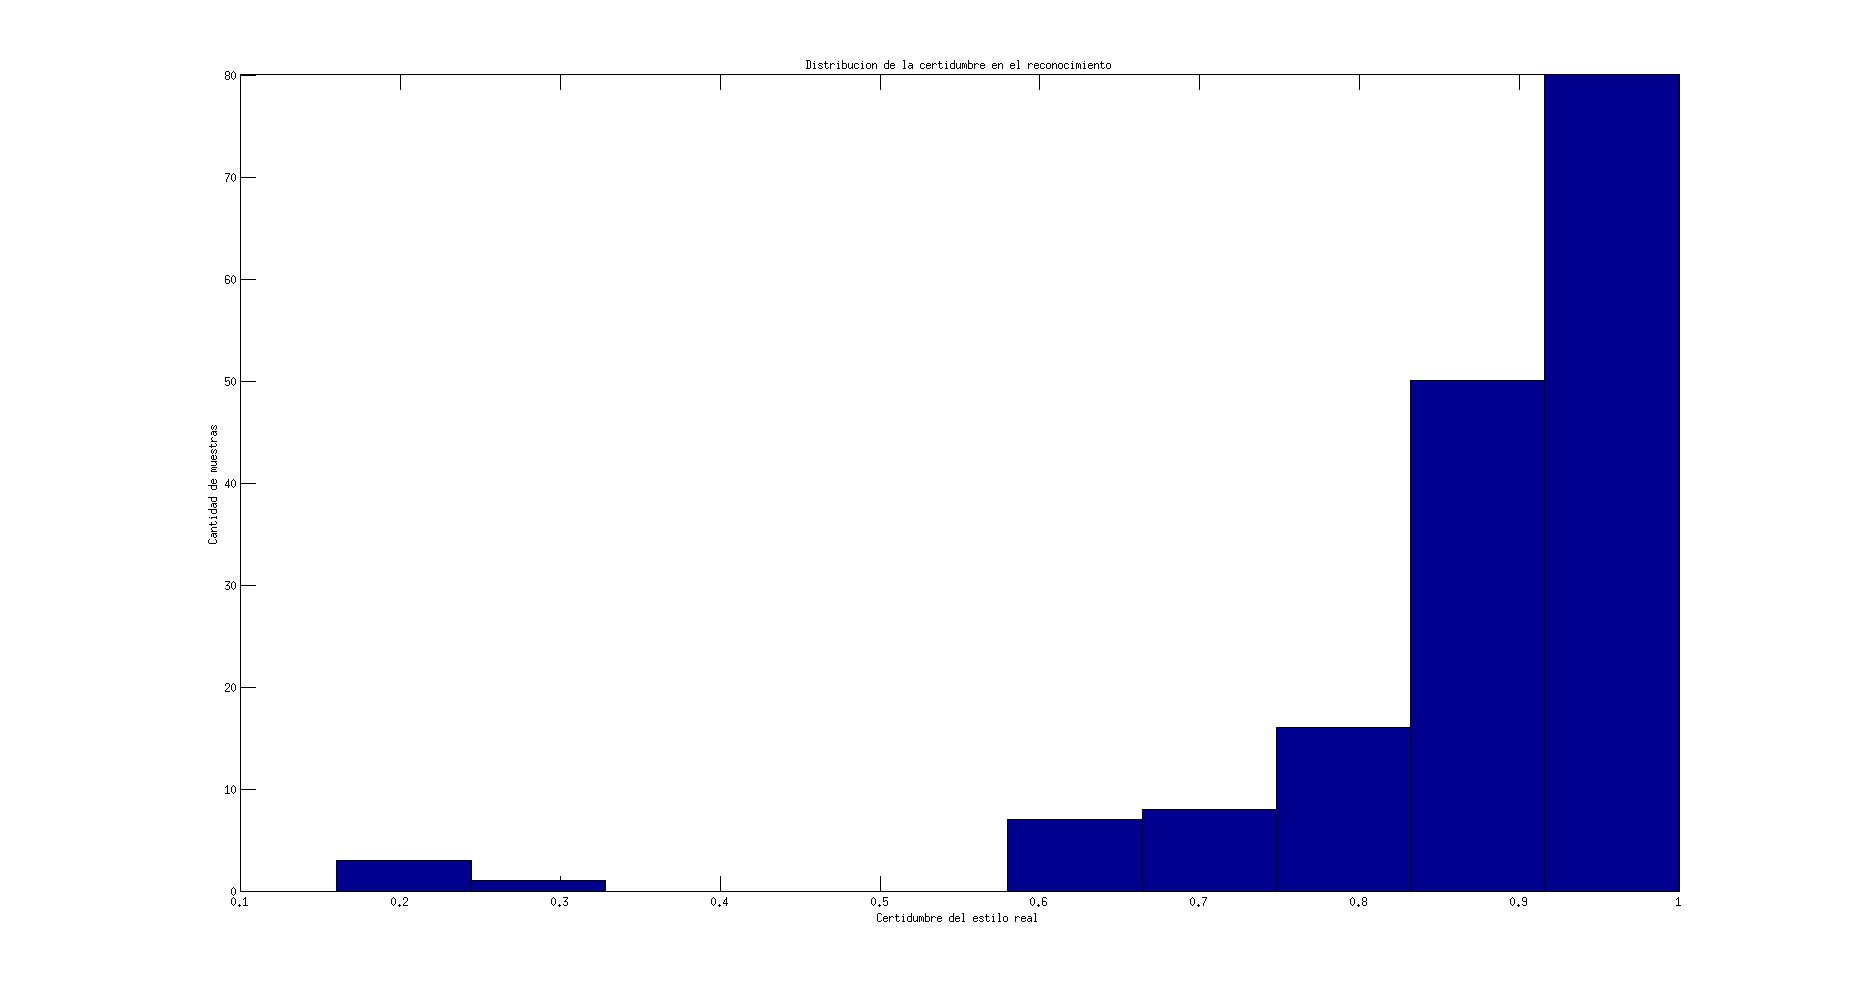
\includegraphics[width=0.9\textwidth]{implementacion/img/fitness_histograma.jpg}
    \caption{Distribución de la certidumbre del conjunto de entrenamiento}
\end{figure}

\begin{center}
    \begin{tabular}{| c | c | c | c |}
        \hline
        \multirow{Interprete} & \multicolumn{3}{|c|}{Similitud media con} \\
         & Frank Sinatra & Elvis Presley & Sex Pistols \\ \hline
        Frank Sinatra & 40.66\% & 59.33\% & 0\% \\  
        Elvis Presley & 2.66\% & 28\% & 69.33\% \\
        Sex Pistols & 77.33\% & 19.33\% & 3.33\% \\
        \hline  
    \end{tabular}
\end{center}